\chapter{Paraphrasing using phrase-based machine translation}
\addcontentsline{toc}{chapter}{moses}

In the following two chapters,\footnote{This chapter is based on the article \citep{barancikova:itat2014}, which is a joint work with Aleš Tamchyna. 
Aleš was in charge of training and tuning Moses. My responsibilities included data preparation, paraphrasing and evaluation of experiments.} 
we present a method of targeted paraphrasing of using machine translation itself. 

There is a strong resemblance between translation and paraphrasing -- they both strive to preserve the meaning of a sentence.  While translation focuses on converting text from one language to another, paraphrasing achieves the same objective within a single language by using a different choice of words.  %\cite{madnani:2010}  
Both processes require a deep understanding of the original content and the ability to convey the intended message accurately while considering linguistic nuances, cultural context, and the target audience. 

Interestingly, machine translation has a wide array of tools and resources available compared to the relatively limited availability of paraphrasing tools. Given this disparity, it appears only logical to leverage existing machine translation engines and adapt them for the purpose of targeted paraphrasing within a single language.
 
We describe this attempt on two types of MT systems -- phrase-based and rule-based. 
Initially, we experiment with the freely available SMT system Moses.
We create its translation model from  Czech paraphrase tables and added a new feature to make the translation targeted.
However, the results of this method are inconclusive. 
In the view of errors appearing in the new paraphrased sentences, we propose another solution -- targeted paraphrasing using parts of a rule-based translation system included in the NLP framework Treex, which easily overcomes some of the problems of Moses. \Sref{treex}
%ing the analysis, we get a representation of the sentence
%on tectogrammatical layer, where we can swap a word and its grammatems for its paraphrase. 
%Then using the synthesis back to the word layer.

%todo

\section{Data} 
We perform our experiments on data from the English-to-Czech translation task 
of WMT12 \cite{wmt12}. 

\section{Moses}
Moses \citep{moses} is a widely recognized open-source statistical machine translation (SMT) engine. It has been a prominent tool in the field of machine translation for several years.
The advancements in neural machine translation (NMT), particularly with the introduction of the Transformer architecture and pre-trained models, have led to significant improvements in translation quality and made NMT the preferred approach for many translation tasks.

Moses generates translatations using statistical models. The translation process involves the following phases: creating language and translation models, parameter tuning and decoding. We use Moses in the phrase-based setting.

The first phase in statistical machine translation is creating language and translation models. 
A language model is responsible for a correct word order and grammatical correctness 
of the translated sentence. A translation model (phrase table) supplies all possible 
translations of a word or a phrase. Models are assigned weights which are learned 
during the parameter tuning phase.

During the decoding phase, all these models are combined to maximize 
$ \sum_i \lambda_i \phi_i (\bar{f},\bar{e}) $, where  $ \lambda_i $ is a weight 
of a the sub-model $ \phi_i $ and $ \bar{f},\bar{e} $ is a hypothesis and source 
sentence, respectively. In our case, we want to make a reference sentence closer
to a corresponding machine translation output -- $ \bar{e} $ is the reference 
sentence and $ \bar{f} $ is a new synthetic reference.

On its own, this setting could create paraphrases, but they would be just random
paraphrases of the reference sentence -- their similarity in wording to our original 
hypotheses would not be guaranteed. Therefore, we also add a new feature for targeted 
paraphrasing to Moses.


After building the models, the next phase is parameter tuning. This step involves adjusting the model parameters to optimize the translation quality. Various optimization techniques, such as minimum error rate training or maximum likelihood estimation, are employed to fine-tune the statistical models.

Finally, the decoding phase takes place. In this stage, the models are used to generate translations for input sentences. The input sentence is segmented into phrases, and the translation model scores different translation options for each phrase. The decoding algorithm then searches for the most probable translation by considering both the translation model scores and the language model probabilities. The resulting translation is the output of the decoding process.

When it comes to Moses, it is specifically used in the phrase-based setting. The phrase-based approach to machine translation divides the input sentence into smaller units, or phrases, and translates them independently. These translated phrases are then recombined to form the final translation. Moses excels in this setting, providing efficient and effective translation capabilities.


\subsection{Language model}
We create the language model (LM) using the SRILM toolkit \cite{srilm} on the 
data from the Czech part of the Czech-English parallel corpus CzEng \cite{czeng}. 

\subsection{Phrase models}

\begin{table*}[ht]
%\begin{center}
\begin{tabular}{r|l|c|c}
setting & reference sentence used & correlation & avg. BLEU \\
\hline
\textbf{Baseline} & original reference sentence, no paraphrasing & \textbf{0.75} & 12.8 \\
\textbf{Paraphrased} & paraphrased by Moses using MERT-learned weights  & 0.50  & 15.8 \\
\textbf{LM+0.2}  & paraphrased by Moses with LM weight increased by 0.2  & 0.24 & 9.1 \\
\textbf{LM+0.4} & paraphrased by Moses with LM weight increased by 0.4  & 0.22 & 6.7 \\
\end{tabular}
\caption{Description of basic settings and the results - Pearson's correlation of BLEU and the
human judgment, the average BLEU scores.} 
%korelace metrik - 0.981
\label{settings}
%\end{center}
\end{table*}
\begin{figure*}[htb]
\begin{center}
\begin{tabular}{l|r}
 \textbf{Source } &  \textit{Paclík claims he would dare to manage the association.} \\
 \hline
 
 \textbf{Baseline} & Paclík tvrdí , že by si na vedení asociace troufl.\\
           & \textit{Paclík claims he would dare to lead the association.} \\

 \hline
 \textbf{Hypothesis} & Paclík tvrdí, že by se odvážil k řízení komory. \\
            & \textit{Paclík claims he would find the courage to control the chamber.}  \\ 

 \hline
 \textbf{Paraphrased} & Paclík tvrdí, že by se na řízení organizace troufl. \\
             & \textit{*Paclík claims he would dare to control the organization.}\\
 \hline 
 \textbf{LM+0.2} & Paclík tvrdí, že by si troufl na řízení ekonomiky. \\
               &\textit{ Paclík claims he would dare to control the economy.} \\
  
\hline 
 \textbf{LM+0.4} & Říká se, že Paclík si troufl na řídící rady. \\
               & \textit{They say that Paclík ventured to governing boards.} \\
%Lexical & Paclík tvrdí , že by se na řízení asociace troufl .\\
%Lexical boosted by 20 & Paclík tvrdí , že by si troufl na řízení ekonomiky .\\
%asociace, komora nikde nejsou jako parafraze

\end{tabular}
\caption{Example of the targeted paraphrasing. The~hypothesis is grammatically 
correct and has very similar meaning as the source sentence. The new reference 
is closer in wording to the hypothesis, but there is an error in a word choice. 
The sentences created with increased weights of the language model are both 
grammatically correct, but the sentence lost its original meaning.}
\label{example}
\end{center}
\end{figure*}

Each entry in Moses phrase tables contains a phrase, its translation, several
feature scores (translation probability, lexical weight etc.), and optionally
also alignment within the phrase and frequencies of phrases in the training data.
The phrase tables are learned automatically from large parallel data.
As we do not have any large corpora of Czech-Czech parallel data, we create the 
following two ``fake'' translation models for paraphrasing from our paraphrase 
tables. 

\begin{itemize}
\item \textbf{Enhanced Meteor tables}\\
This table was created from the Czech Paraphrase Meteor table. It was constructed
via \textit{pivoting}. \cite{pivoting} The pivot method is an inexpensive way of 
acquiring paraphrases from large parallel corpora. It is based on the assumption 
that two phrases that share a meaning may have a same translation in a foreign 
language. \cite{dyvik}

Each paraphrase pair comes with a pivoting score which we adapt as a feature in 
out phrase table. However, this score turns out to be even worse then random 
selection \cite{barancikova:2014}, so we do not expect it to get a high weight 
in tuning.

For that reason, we add our own paraphrase scores, acquired by \textit{distributional
semantics}. Distributional semantics assumes that two phrases are semantically 
similar if their contextual representations are similar. \cite{miller-91}

We collect all contexts (words in a window of limited size) in which Meteor 
paraphrases occur in the Czech National Corpus \cite{SYN2010} and then measure 
context similarity (cosine distance, taking into account the number of word 
occurrences) for each pair of paraphrases. 

We add six scores for each pair of paraphrases according to the size of the 
context window used (1-3 words) and whether word order played a role in the 
context. 

\item\textbf{One-word paraphrase table}\\
We first create a set of all words from Czech side of CzEng appearing at least
five times to exclude rare words and possible typos. We also add all words appearing 
in the MT outputs and the reference sentences. Morphological analysis of the words was
then performed using Morče. 

For every word $ x $ from this set, we add to this translation table every pair of 
words that fulfills at least on of the following requirements:

\begin{itemize}
\item $ x,x $ (not every word should be paraphrased)
\item $ x,y $, if lemma of $ x $ is lemma of $ y $ (some word 
might have different morphology in the paraphrased sentence)
\item $ x,y $, if lemma of $ x $ and lemma of $ y $ are paraphrases according 
to Czech WordNet PDT 1.9.
\item $ x,y $, if lemma of $ x $ and lemma of $ y $ are paraphrases according 
to the filtered Meteor.
\end{itemize}

These categories constitute the first four scores in the phrase table. A pair of 
words gets score $ e $ if they fall in a given category, 1
($e^0$) otherwise.\footnote{Phrase-table scores are considered log-probabilities.} 
This phrase table contains more than 1,100k pairs of words.

We add another score expressing POS tag similarity between the two words. It is computed 
$ e^{\frac{1}{a+1}}$, where $ a $ is the minimal Hamming distance between tags of the
words. This probability should reflect how morphologically distant the paraphrases are. 
\end{itemize}

\subsection{Feature for targeted paraphrasing}
In order to steer the MT decoder (translation engine) in the direction of the
hypotheses, we implemented an additional feature for Moses which
measures the overlap with the hypothesis. In order to keep its computation
tractable during search, the overlap is defined simply as the number of words
from the hypothesis confirmed by the reference translation.

Integration into the beam search algorithm used in phrase-based decoding
requires us to keep track of feature state (i.e. reference words covered) to
allow for correct hypothesis recombination. We also implemented an estimator of
future phrase score, defined as the number of reference translation words
covered by the given phrase. Our code is included in
Moses.\footurl{https://github.com/moses-smt/mosesdecoder/}

\subsection{Parameter tuning}
We use the minimum error rate training (MERT) \cite{mert} to find the optimal 
weights for our models. MERT asserts the weights to maximize the translation 
quality, which is measured with BLEU. We employ the reference sentences and the 
highest rated MT output as the parallel data for tuning. 

This method, however, turned out not to be optimal for our setting. Our feature for 
targeted paraphrasing naturally obtains the highest weight as it provides an oracle 
guide towards the hypothesis.

Other important models, e.g. the language model, get comparably very small weights. The 
paraphrased sentences tend to be closer to the hypothesis, but not grammatically correct. 
Therefore, we experiment with increasing the weight of the language model manually. 

\begin{table*}[tb]
\begin{center}
\begin{tabular}{r|l|c|c}
\hline
setting & reference sentence used & correlation & avg. BLEU \\
\hline
\textbf{Lexical} &  Only one-word paraphrase table & 0.56 & 15.1 \\
\textbf{Lexical \& LM+0.2}  & \textbf{Lexical} and LM weight increased by 0.2 & 0.33  & 9.5 \\
\textbf{Monotone}  & \textbf{Lexical} and monotone translation & \textbf{0.61} & 18.1 \\
\end{tabular}
\caption{Additional settings and the results -- Pearson's correlation and the average BLEU scores.} 
\label{settings2}
\end{center}
\end{table*}

%Vahy
%Distortion0= 0.0263445
%LM0= 0.0159449
%CoveredReferenceFeature0= 0.513121
%WordPenalty0= 0.291437
%PhrasePenalty0= 0.00566341
%TranslationModel0= 0.024998 -0.00344275 0.0206294 0.00278498 0.0305869
%TranslationModel1= 0.010452 -0.0219544 0.00883162 0.00627672 -0.00401715 0.0111173 0.00239786

%\xxx{tu je mnoho uzitecneho!/home/barancikova/WORK/moses/tables }

\section{Results}

We compare four different basic settings, the results are presented in \Tref{settings}
as the Pearson’s correlation coefficient of BLEU and the human judgment. 
A visualization of the results is shown in \Fref{visualization}. The baseline
score is not exceeded by any of our paraphrasing methods, in contrast to  our previous 
results (\cite{parmesan}, \cite{barancikova:2014}). 

There are several reasons for the clear decrease in correlation with paraphrased 
references. Hypotheses generated by the \textbf{Paraphrased} setting, while obtaining 
a significantly higher BLEU score, were mostly ungrammatical and reduced the 
correlation of our metric.

The small weight of the language model seems to be the problem, but its increase brings
even more chaos. It creates hypotheses which are nice and grammatically correct 
but often wholly unrelated to the source sentence.

This shows that our paraphrase table noise filtering was by no means sufficient and
there is still a lot of noise in our phrase tables. Furthermore, the MT output
might be far from being a correct sentence -- given the high weight for the targeted 
paraphrase feature, we essentially transform the correct reference 
sentences to incorrect hypotheses at all cost, using our noisy phrase tables.

Our targeting feature is also not ideal -- it ignores word order and operates
only on the word level (it does not model phrases). Ungrammatical translations
with scrambled word order are considered perfectly fine so long as the
translation contains the same words as the reference. So while the feature does
provide a kind of oracle, it does not guarantee reaching the best possible
translation in terms of BLEU score, let alone a grammatical translation.

Another problem is illustrated by very small weights assigned to our translation
models. In fact, the highest weight was assigned to the tag similarity feature.
This shows that our model features (Meteor score and distributional
similarity scores) fail to distinguish good paraphrases from the noise. 

The combination of noise in the translation tables and the boosted language
model then caused that during the decoding phase, the most common paraphrase
according to the language model with a similar tag got the preference. 

\Fref{example} represents an example of our paraphrasing method. The~hypothesis is 
grammatically correct and has a very similar meaning as the reference sentence. The 
new paraphrased reference is slightly closer in wording to the hypothesis, but there 
is an error due to a bad word choice. The boosted language model reduces errors, 
however the meaning of the sentences is shifted. In the \textbf{LM+0.4} setting, 
they also differ a lot in wording from both the hypothesis and the reference sentence.


\begin{figure*}[htb]
\begin{center}
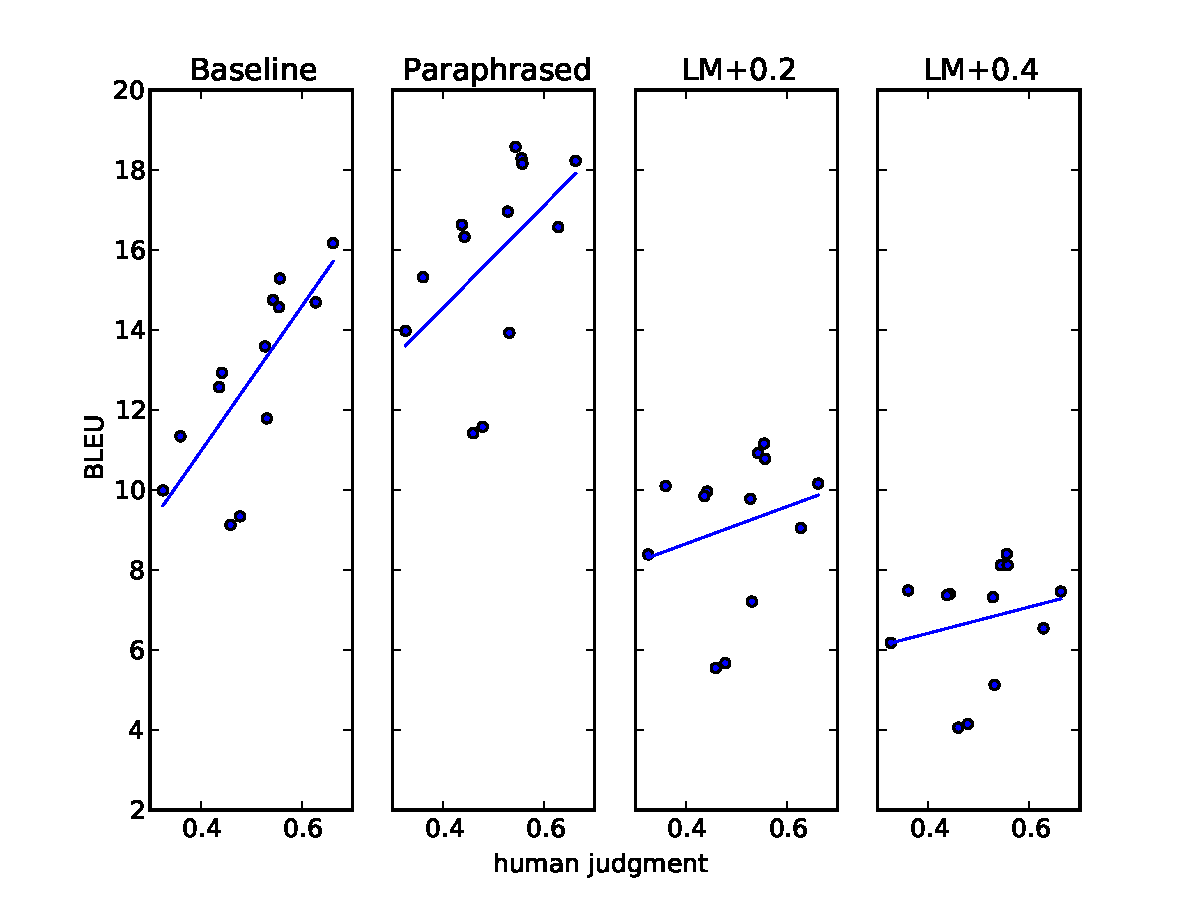
\includegraphics[scale=0.6]{../img/moses_multigraf.pdf}
\caption{Visualization of BLEU and human judgment for the four basic settings. 
We add the linear regression lines to better demonstrate the linear correlation.}
\label{visualization}
\end{center}
\end{figure*}
 
Based on such poor results, we decided to experiment with three more settings 
(see \Tref{settings2}). We omit the Enhanced Meteor tables as they brought
most of the noise to the translation. One of the common errors using the 
\textbf{Paraphrased} setting is scrambled word order (often, punctuation
appeared in the middle of the sentences).
We attempt to fix that by using monotone translation (i.e. by disabling reordering).

These constraints improve the correlation with human judgment. However, they still
do not overcome the baseline results.

\section{Conclusion}
We experiment with paraphrasing using the phrase-based machine translation system 
Moses. We show that it is a universal tool that can be used for other purposes than
machine translation directly. Within Moses, we introduced a new feature for targeted 
paraphrasing and artificial phrase tables for paraphrasing. 

However, our results are inconclusive and the correlation with human judgment
drops. It is caused mainly by the high amount of noise in our translation tables and
not well balanced trade-off between paraphrasing and the language model.


\section{Future Work}
% better setting of weights
Based on our results, Moses does not seem to be the optimal tool for our task, especially
unless we have at our disposal better paraphrasing tables. A new paraphrase database 
PPDB \cite{GANITKEVITCH14} for Czech language should be released any time now. 

Furthermore, there may be a better solution than a phrase-based translation
system, namely Treex \cite{treex}, a highly modular NLP software system. Treex
was developed for TectoMT, which is a rule-based machine translation system that
operates on deep syntactic layer.

Treex implements the stratificational approach to language, adopted from the 
Functional Generative Description theory \cite{FGP} and its later extension by the 
Prague Dependency Treebank \cite{PDT3.0}. It represents sentences in four layers:
word layer, morphological layer, shallow-syntax layer and deep-syntax layer 
(tectogrammatical layer).

We can transfer both hypothesis and reference sentence to the morphological layer, 
where we can extract lemmas that appear in only one of the sentences. Those after
filtering according to our paraphrase tables represent candidates for substitution.
Furthermore, we are able to transfer a reference sentence to a tectogrammatical 
layer, where we can replace individual lemmas from the hypothesis with their paraphrases 
and corresponding grammatemes. Then we transfer the altered reference sentence back to 
the word layer.

This way should easily overcome some of the problems that appear when paraphrasing using 
Moses. First of all, we only compare two sentences and there is less space for %neni treba stavet tabulky
the noise to interfere. Also there is highly developed machinery to avoid ungrammatical 
sentences. We can change only parts of sentences that are dependent on the changed 
word, thus keeping the rest of the sentence correct and creating more conservative 
reference sentences.

